\documentclass[11pt,a4paper]{article}

\usepackage{url}
\usepackage{graphicx}
\title{Raspberry Pi: Establishing Network connection and SSH connection}
\author{e-Yantra Team}
\date{\today}

\begin{document}
	\maketitle
	\newpage
	\tableofcontents
	\newpage
	\section{Objective}
	In this tutorial we will be learning how to establish a network connection in an R-Pi and how to connect a PC to a Raspberry Pi using SSH connection(i.e. remote control).
	\section{Prerequisites}
	One should be aware of :
	\begin{itemize}
		\item Basic terminal commands.
		\item The ssid and password of a wireless network to which an R-Pi has to be connected.
	\end{itemize}
	
	\section{Hardware Requirement}
	\begin{enumerate}
		\item Raspberry Pi (I will be using Version 2 Model B)
		\item Monitor,HDMI cable,Keyboard,Mouse (This an optional mode of connecting an R-Pi.In order to learn about different ways to connect an R-Pi kindly refer the previous tutorial)
		\item Wireless adapter
		\item Power adapter
		\item PC(either Windows or Linux)
	\end{enumerate}
		
	\section{Software Requirement}
	MobaXterm(for Windows user)
	
	\newpage
	\section{Theory and Description}
	Secure Shell is a program to log into another computer over a network, to execute commands in a remote machine, and to move files from one machine to another. It provides strong authentication and secure communications over insecure channels. It is a replacement for rlogin, rsh, rcp, and rdist.
	SSH protects a network from attacks such as IP spoofing, IP source routing, and DNS spoofing. An attacker who has managed to take over a network can only force ssh to disconnect. He or she cannot play back the traffic or hijack the connection when encryption is enabled.
	When using ssh's slogin (instead of rlogin) the entire login session, including transmission of password, is encrypted; therefore it is almost impossible for an outsider to collect passwords. [2]
	\begin{figure}[h!]
		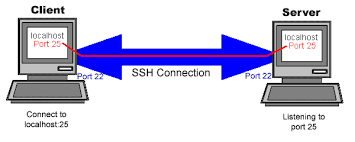
\includegraphics[scale=0.8]{ssh.png}
		\centering
		\caption{[3]}
	\end{figure}
	\textbf{Applications of SSH or OpenSSH protocol}
	\begin{itemize}
		\item For login to a shell on a remote host (replacing Telnet and rlogin)
		\item For executing a single command on a remote host (replacing rsh)
		\item For setting up automatic (passwordless) login to a remote server (for example, using OpenSSH)
		\item Secure file transfer
		\item In combination with rsync to back up, copy and mirror files efficiently and securely
		\item For forwarding or tunneling a port (not to be confused with a VPN, which routes packets between different networks, or bridges two broadcast domains into one).
		\item For using as a full-fledged encrypted VPN. Note that only OpenSSH server and client supports this feature.
		\item For forwarding X from a remote host (possible through multiple intermediate hosts)
		\item For browsing the web through an encrypted proxy connection with SSH clients that support the SOCKS protocol.
		\item For securely mounting a directory on a remote server as a filesystem on a local computer using SSHFS.
		\item For automated remote monitoring and management of servers through one or more of the mechanisms discussed above.
		\item For development on a mobile or embedded device that supports SSH.[1]
	\end{itemize}
	
	\flushleft
	\textbf{MobaXterm}
	\vspace{0.4cm}
	\newline MobaXterm is a tool used for remote computing. In a single Windows application, it provides loads of functions that are tailored for programmers, webmasters, IT administrators and pretty much all users who need to handle their remote jobs in a more simple fashion.It provides all the important remote network tools (SSH, X11, RDP, VNC, FTP, MOSH, ...) and Unix commands (bash, ls, cat, sed, grep, awk, rsync, ...) to Windows desktop, in a single portable exe file which works out of the box. \newline
	
	There are many advantages of having an All-In-One network application for your remote tasks, e.g. when you use SSH to connect to a remote server, a graphical SFTP browser will automatically pop up in order to directly edit your remote files. Your remote applications will also display seamlessly on your Windows desktop using the embedded X server.[4]
		
	\newpage
	\section{Experiments}
	
	\subsection{Establishing a network connection}
	Before we can start using a Raspberry Pi remotely we need to configure its network settings.There are two ways to configure network setting:
	\begin{itemize}
		\item One is using DHCP server (wireless connection)
		\item The other one is by assigning a static IP
	\end{itemize}
	
	\subsubsection{Network settings configuration using DHCP Server(wireless settings)} 
	\begin{enumerate}
		\item Insert the SD card (with Raspbian OS already written) into the micro SD slot in an R-Pi.
		\item Connect the wireless adapter, keyboard , mouse and monitor (using a HDMI cable) to the Raspberry Pi.
		\item Power on the board and monitor.You will notice a set of code running on the monitor.
		\item Enter the set user name and password and then type \textit{startx} command to launch the GUI.
		\begin{figure}[h!]
			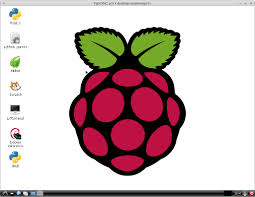
\includegraphics[width=10cm]{r1.jpg}
			\centering
		\end{figure} 
		\item Click on the icon at the bottom-left on the screen. This is the start icon.
		\item Select LXTerminal option to open a terminal window
		\newpage
		\begin{figure}[h!]
			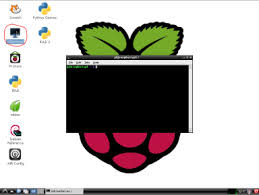
\includegraphics[width=10cm]{lxt.jpg}
			\centering
		\end{figure}
		\item Some of the previous versions of Raspbian OS do not support wireless module. To know about the version you are using type \textit{uname -a}. To upgrade to the latest one type "sudo apt-get upgrade".
		\item Connect your wireless adapter . To check if its connected type \textit{lsusb}(We used D-link adapter which is highlighted in yellow) 
		\begin{figure}[h!]
			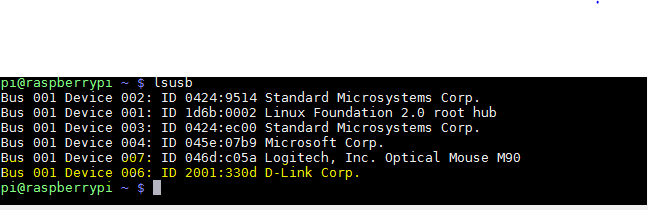
\includegraphics[scale=0.6]{Lsusb.PNG}
			\centering
		\end{figure}
		\item Now type \textit{sudo nano /etc/network/interfaces} and press enter. You will see the following window:
		\newpage
		\begin{figure}[h!]
			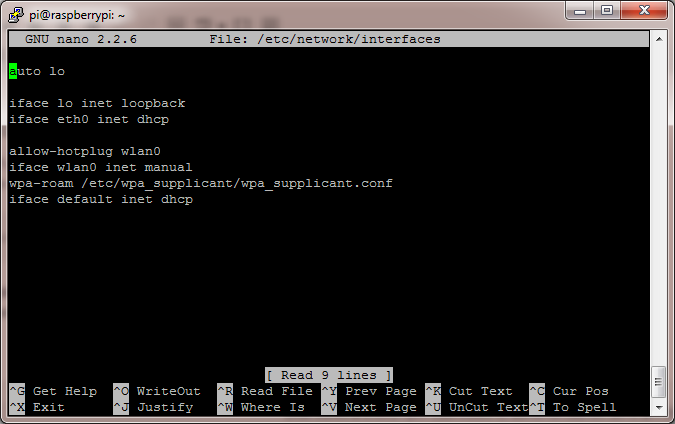
\includegraphics[scale=0.6]{iwifi.png}
			\centering
		\end{figure}
		\item Change the code by adding the following lines:
		\begin{figure}[h!]
			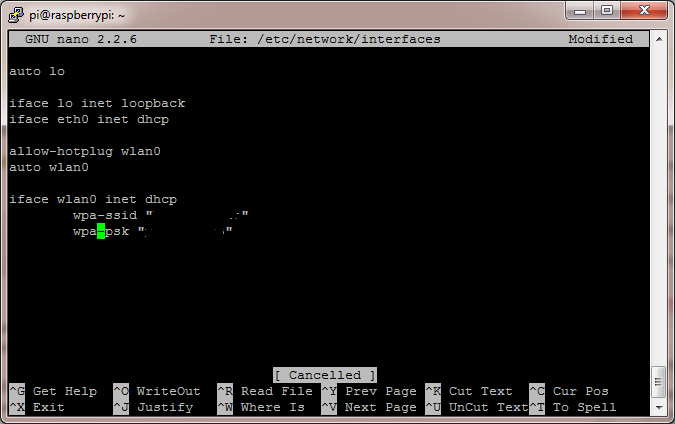
\includegraphics[scale=0.6]{wificon.png}
			\centering
		\end{figure}
		\item Add in the SSID(username) and Password of your wifi. Then for changes to take effect type \textit{sudo /etc/init.d/networking restart} 
		\item Type \textit{ifconfig} to obtain the IP address of R-Pi etc. It will be under wlan0(written as inet address).
	\end{enumerate}
	
	\newpage
	\subsubsection{Network settings using static IP method}
	The router normally distributes the dynamic IP addresses but it isn’t guaranteed that it will assign the same IP address every time. This can cause problems if you are trying to connect to your Raspberry Pi remotely. And hence we can assign a static IP. In order to do so follow these steps:
	\begin{enumerate}
		\item Open the LXTerminal and type the following command \newline \textit{cat /etc/network/interfaces}
		\item Before you make changes to the document you should be aware of your current IP address, the broadcast IP and the Mask Use the command \textit{ifconfig} to retrieve this information
		To find your gateway address type the following command: \textit{sudo route \-nee}
		\item In order to edit the interfaces file type \textit{sudo nano /etc/network/interfaces}
		\item Remove the following line \textit{iface eth0 inet dhcp} and add the following:\newline \textit{iface eth0 inet static \newline address 192.168.0.x \newline netmask 255.255.255.0 \newline network 192.168.0.0 \newline broadcast 192.168.0.255 \newline gateway 192.168.0.y }
	    \item Save the file using Ctrl+X, Y.
	    \item For changes to take effect type \textit{sudo /etc/init.d/networking restart} and reboot the system.
    \end{enumerate}
	
	
	\newpage	
	\subsection{Establishing an SSH connection}
	
	To start using a Raspberry Pi remotely follow these steps:
	\begin{enumerate}
		\item A windows user should download MobaXterm (latest version) using the following link: \url{http://mobaxterm.mobatek.net/}
		\item Run the .exe file and open the application.
		\begin{figure}[h!]
			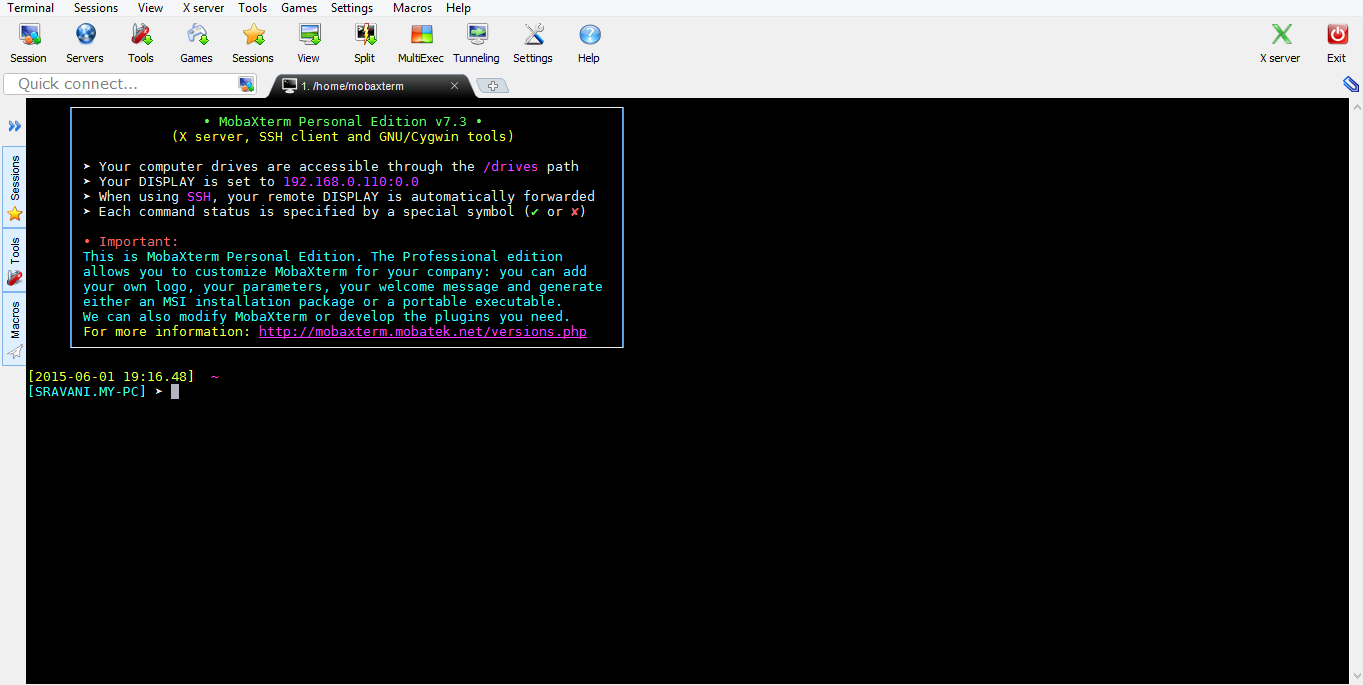
\includegraphics[scale=0.3]{M1.PNG}
			\centering
		\end{figure}
		\item Then select the session option on the toolbar.
		\begin{figure}[h!]
			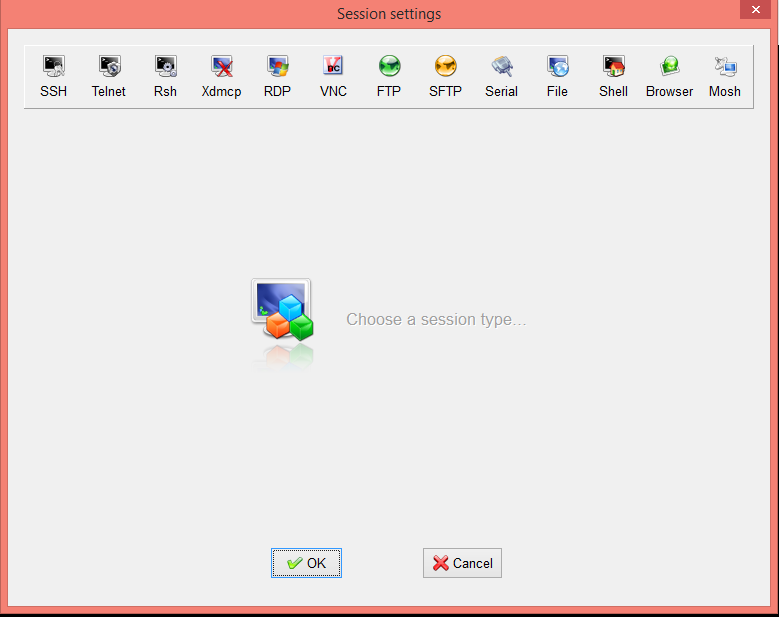
\includegraphics[scale=0.5]{M2.PNG}
			\centering
		\end{figure}
		\newpage
		\item Click on the SSH option. A settings window opens as shown
		\begin{figure}[h!]
			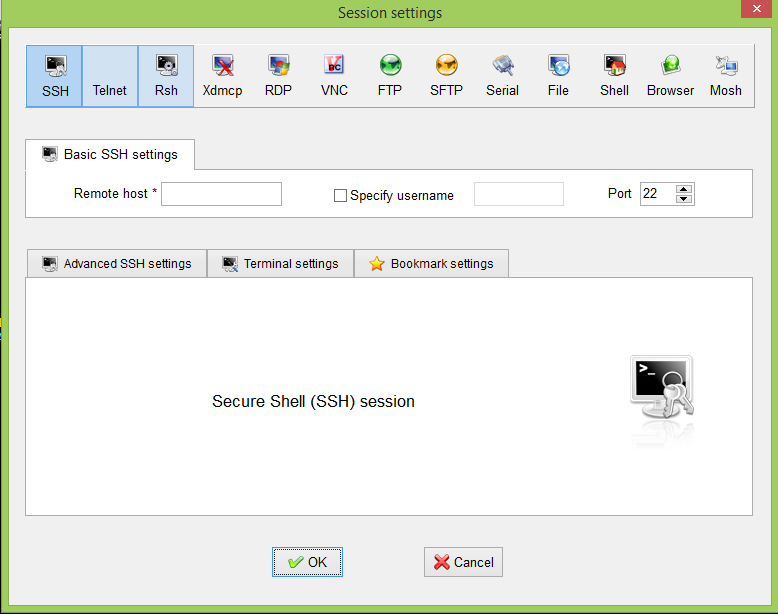
\includegraphics[scale=0.5]{M3.PNG}
			\centering
		\end{figure}
		\item Enter the IP address of the R-pi in the Remote host field and in the 'Advanced SSH settings' option configure the remote environment either as 'Interactive shell (terminal based)' or as an 'LXDE desktop(GUI based)'and click OK
		\item If you are using the Interactive shell environment login to the R-Pi using the following command: ssh -X pi@192.168.0.4 (IP address of pi) and then enter the login id and password to start using the Pi remotely.
		\item If you are using the LXDE desktop i.e. the GUI environment then use LX terminal icon to start programming the Pi.
		\begin{figure}[h]
			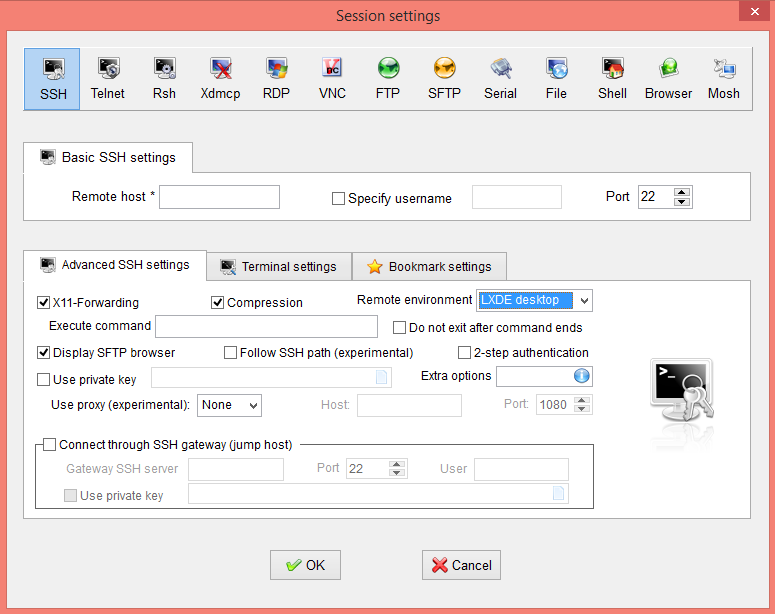
\includegraphics[scale=0.5]{M4.PNG}
			\centering
		\end{figure}
		\newpage
		\item Also the established session is saved. So the next time you want to access directly click on the R-Pi's address mentioned in the saved session option to start using the Pi remotely.
		\begin{figure}[h!]
			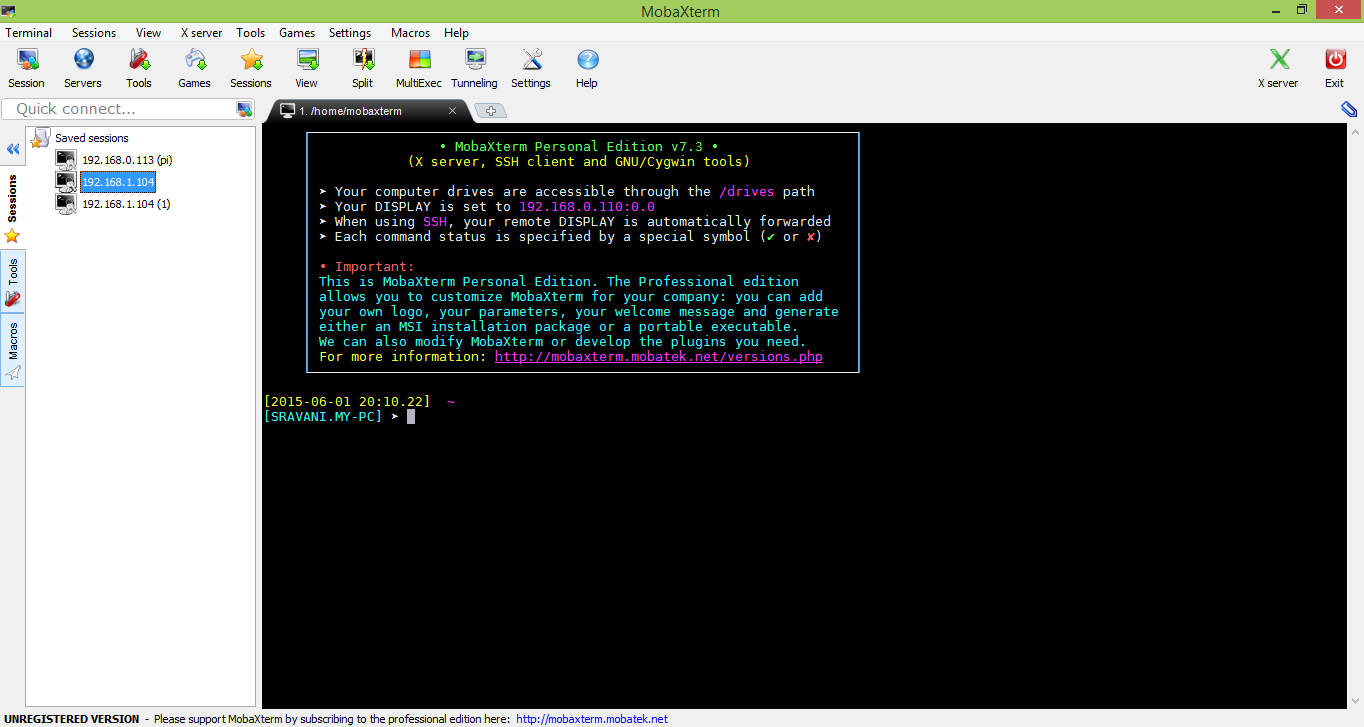
\includegraphics[scale=0.3]{M5.PNG}
			\centering
		\end{figure}
	\end{enumerate}

	\textbf{Note:} A linux user needn't download any Xterm file. They can directly start accessing the R-Pi using the command: ssh -X pi@192.168.0.4 (IP address of pi) and then entering the login id and password for using the Pi remotely.
	
	\newpage
	\section{References}
	\begin{enumerate}
		\item \url{http://en.wikipedia.org/wiki/Secure_Shell}
		\item \url{http://www.webopedia.com/TERM/S/SSH.html}
		\item \url{http://www.codemastershawn.com/library/tutorial/images/ssh.tunnel.overview.gif}
		\item \url{http://mobaxterm.mobatek.net/}
		\item \url{http://www.suntimebox.com/raspberry-pi-tutorial-course/week-3/day-5/}
	\end{enumerate}
\end{document}



